\chapter{Protezione}
    
\subsubsection{Sicurezza}
Insieme delle tecniche per regolamentare l'accesso degli utenti al sistema di elaborazione. La sicurezza impedisce accessi non autorizzati al sistema e i conseguenti tentativi dolosi di alterazione e distruzione dei dati.

Meccanismi per \textbf{identificazione}, \textbf{autenticazione} e \textbf{autorizzazione} di utenti "fidati".
    	
\subsubsection{Protezione}
Insieme di attività volte a garantire il controllo dell'acecsso alle risorse logiche e fisiche da parte degli utenti autorizzati all'uso di un sistema di calcolo.

Definizione, per ogni utente autorizzato, di:
\begin{itemize}
	\item quali \textbf{risorse} sono accessibili
	\item quali \textbf{operazioni} può effettuare
\end{itemize}

Sono stabilite tramite tecniche di controllo degli accessi.

\section{Protezione}
In un sistema, il controllo degli accessi si esprime tramite la definizione di tre livelli concettuali:
\begin{itemize}
	\item modelli
	\item politiche
	\item meccanismi
\end{itemize}

\subsection{Modelli}
Un modello di protezione definisce \textbf{soggetti}, \textbf{oggetti} ai quali i soggetti possono accedere e i \textbf{diritti} di accesso:
\begin{itemize}
	\item oggetti, risorse fisiche e logiche alle quali applicare limitazione di accesso;
	\item soggetti, entità che possono richiedere l'accesso agli oggetti, utenti e processi;
	\item diritti di accesso, operazioni con le quali è possibile operare sugli oggetti;
\end{itemize}

\subsubsection{Dominio di protezione}
Ad ogni soggetto è associato un \textbf{dominio} che rappresenta l'ambiente di protezione nel quale il soggetto esegue, il dominio specifica i diritti di accesso posseduti dal soggetto nei confronti di ogni risorsa.

Un dominio di protezione è \textbf{unico per ogni soggetto}, mentre un processo può eventualmente cambiare dominio durante la sua esecuzione.

\subsection{Politiche}
Le \textbf{politiche di protezione} definiscono le regole con le quali i soggetti possono accedere agli oggetti.

Classificazione delle politiche:
\begin{itemize}
	\item \textbf{Discetional Access Control} (DAC): il creatore di un oggetto controlla i diritti di accesso per quell'oggett (UNIX), definzione delle politiche decentralizzata.
	\item \textbf{Mandatory Access Control} (MAC): i diritti di accesso vengono definiti in modo centralizzato. Installazione ad alta sicurezza (es. enti gonvernativi)
	\item \textbf{Role Based Access Control} (RABC): un ruolo ha specifici diritti di accesso alle risorse, gli utenti possono appartenere a diversi ruoli, i diritti sono assegnati in modo centralizzato.
\end{itemize}

\subsubsection{Principio del privilegio minimo}
Ad ogni soggetto sono garantiti i diritti di accesso solo agli oggetti strettamente necessari per la sua esecuzione, è una caratteristica desiderabile in tutte le politiche di protezione.

\subsection{Meccanismi}
I meccanismi di protezione sono gli strumenti messi a disposizione dal sistema di protezione per imporre una determinata politica.

\subsubsection{Principi di realizzazione}

\begin{itemize}
	\item \textbf{Flessibilità} del sistema di protezione, i meccanismi di protezione devono essere sufficientemente generali per consentire l'applicazione di diverse politiche;
	\item \textbf{Separazione} tra meccanismi e politiche, la politica definisce il \textit{cosa} va fatto e il meccanismo il \textit{come} va fatto.
\end{itemize}

In UNIX si utilizza la politica DAC e il SO offre un meccanismo per definire e interpretare i tre bit dei permessi.

\subsection{Dominio di protezione}
Un dominio definisce una serie di coppie che associano un oggetto all'insieme delle operazioni che il soggetto associato al dominio può eseguire.

Ogni dominio è associato univocamente a un soggetto.

\subsubsection{Domini disgiunti o con diritti di accesso comune}

Esiste la possibilità per due o più soggetti di effettuare alcune opezione comuni su un oggetto condiviso, le operazioni vengono svolte da processi che operano per conto di soggetti, tuttavia un processo appartiene a un solo dominio in ogni istante.

\subsubsection{Associazione tra processo e dominio}

\paragraph{Modalità statica}
L'insieme di risore disponibili a un processo rimane \textbf{statico} durante tutto il suo tempo di vita.

L'associazione statica non è adatta nel caso si voglia limitare per un processo l'uso delle risorse a quello strettamento necessario.

\paragraph{Modalità dinamica}
L'associazione tra processo e dominio varia durante l'esecuzione del processo.

\subsubsection{Matrice degli accessi}

Un sistema di protezione può essere rappresentato a livello astratto utilizzando una \textbf{matrice degli accessi}.

\begin{figure}[H]
	\caption{Matrice degli accessi}
	\centering
	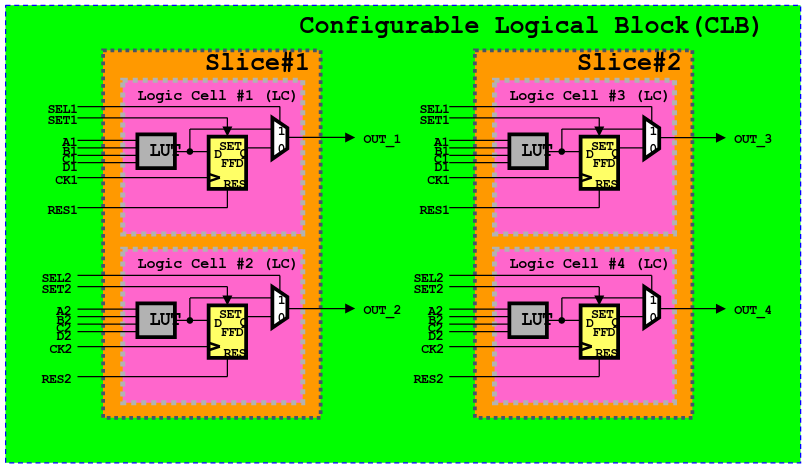
\includegraphics[width=0.8\textwidth]{/home/riccardoob/appunti/sistemi_operativi/images/8.png}
\end{figure}
\begin{itemize}
	\item Ogni riga è associata a un oggetto
	\item Ogni colonna è associata a un oggetto
\end{itemize}

La matrice consente di rappresentare il modello e le politiche valide nel sistema considerato, specificando
\begin{itemize}
    \item \textbf{soggetti}
    \item \textbf{oggetti}
    \item \textbf{diritti} accordati ai soggeti sugli oggetti
\end{itemize}

Le informazioni contenute nella matrice possono variare nel tempo, per effetto di operazioni che ne consentono la modifica $\rightarrow$ le informazioni contenute nella matrice all'istante t rappresenta lo \textbf{stato di protezione} del sistema in t.

La matrice degli accessi offre ai \textbf{meccanismi} di protezione le informazioni che consentono di verificare il rispetto dei vincoli di accesso.

Il meccanismo di protezione:
\begin{itemize}
    \item verifica se ogni richiesta di accesso che proviene da un processo che opera in un determinato dominio è consentita oppure no
    \item autorizza l'esecuzione delle richieste se permesse
    \item esegue la modifica dello stato di protezione in seguite ad ogni richiesta autorizzata da pate di un processo
\end{itemize}

Quando un operazione $M$ deve essere eseguita nel dominio $D_i$ sull'oggetto $O_j$, il meccanismo consente di controllare che $M$ sia contenuta nella casella \texttt{access(i,j)}.  

\subsection{Modello di Graham-Denning}
La modifica controllata dello stato di protezione può essere ottenuta tramite un opportuno insieme di comandi (Graham e Denning, 1972):
\begin{itemize}
    \item create object
    \item delete object
    \item create subject
    \item delete subject
    \item read access right
    \item grant access right
    \item delete access right
    \item transfer access right
\end{itemize}

\subsubsection{Propagazione dei diritti di accesso}
La possibilità di copiare un diritto di accesso per un oggetto da un dominio ad un altro della matrice di accesso è indicato con il \underline{copy flag \texttt{*}}.

Un soggetto $S_i$ può trasferire un diritto di accesso $\alpha$ per un ogget $X$ ad un altro soggetto $S_j$ ad un altro soggetto $S_j$ solo se $S_i$ ha accesso a $X$ con il diritto $\alpha$, e $\alpha$ ha il copy flag.

L'operazione di propagazione può essere realizzata in due modi:
\begin{itemize}
    \item trasferimento del diritto, viene perso dal soggetto originale
    \item copia del diritto: viene mantenuto dal soggetto originale
\end{itemize}

\subsubsection{Diritto owner}
Se un soggetto $S_i$ ha il diritto \textbf{owner} su un oggetto $X$, può assegnare/revocare un qualunque diritto di accesso a un soggetto $S_j$.

\subsubsection{Diritto control}
Se un soggetto $S_i$ ha il diritto \textbf{control} su un soggetto $S_j$, può assegnare/revocare un qualunque diritto di accesso a un soggetto $S_j$ per un qualsiasi oggett $X$.
\begin{figure}[H]
    \caption{Matrice degli accessi}
    \centering
    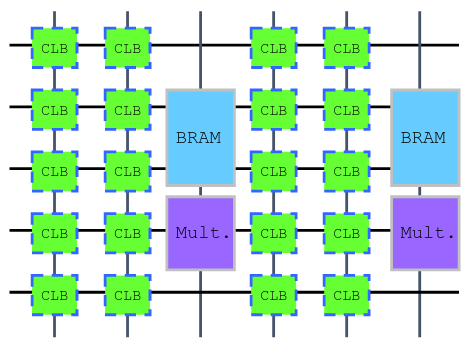
\includegraphics[width=0.6\textwidth]{/home/riccardoob/appunti/sistemi_operativi/images/9.png}
\end{figure}

\subsubsection{Switch}
Un processo che esegue nel dominio del soggetto può commutare al dominio di un altro soggetto $S_j$. L'operazione è consentita solo se il diritto \textbf{switch} appartiene a \texttt{access($S_i$,$S_j$)}.

\subsection{Realizzazione della matrice degli accessi}
La matrice degli accessi è una notazione astratta, realizzare in memoria una struttura dati matriciale $N_s \times N_o$ non sarebbe ottimale, considerando il fatto che è una matrice sparsa.

Esistono due approcci possibili:
\begin{itemize}
    \item \textbf{Access Control List} (ACL): rappresentazione per colonne, ogni oggetto possiede una lista che contiene tutti i soggetti che possono accedervi, con relativi diritti di accesso.
    \item \textbf{Capability List}: Rappresentazione per righe, ogni soggetto possiede una lista che contiene gli oggetti accessibili, con relativi diritti di accesso.
\end{itemize}

\subsubsection{Access control list}
La lista degli accessi, per ogni oggetto, è rappresentata da un insieme di coppie:

{\centering
\texttt{<soggetto, insieme dei diritti>} \par}   

limitatamente ai soggetti con un insieme non vuoto di diritti per l'oggetto.

Quando si deve eseguire l'operazione $M$ su un oggetto $O_j$ da parte di $S_i$, si cerca nella lista degli accessi 

{\centering
\texttt{<$S_i$,$R_k$>}, con $M$ appartente a $R_k$\par}   

La ricerca può essere fatta in precedenza su una lista di default che contiene i diritti di accesso applicabili a tutti gli oggetti.

\paragraph{Utenti e gruppi} Solitamente ogni soggetto rappresenta un singolo utente, molti sistemi tuttavia hanno il concetto di \textbf{gruppo di utenti}, liste di utenti identificate da un nome ch e possono essere inclusi nell'ACL.

Se i gruppi sono presenti, l'ACL ha la seguente forma:

{\centering
$UID_1$ $GID_1$: \texttt{<insieme di diritti>} \par}   

con UID \underline{user identifier} e GID \underline{group identifier}.

\subsubsection{Capability list}
La lista delle capability, per ogni soggetto, è la lista di elementi ognuno dei quali:
\begin{itemize}
    \item è associato a un oggetto a cui il soggetto può accedere
    \item contiene i diritti di accessi consentiti su tale oggetto
\end{itemize}
ogni elemento della lista prende il nome di \textbf{capability} .

La capability si compone di un identificatore (indirizzo) che identifica l'oggetto e la rappresentazione dei vari diritti concessi.

Quando $S$ intende eseguire una operazione $M$ su $O_j$, il meccanismo di protezione controlla se tra le capability di $S$ ne esista una relativa ad $O_j$ che contiene $M$

Le liste di capability devono essere protette da manomissioni, proprietà ottenibile spostando l'effettiva lista nello spazio del kernerl e esponendo soltato un riferimento a tale lista.

L'utilizzo di una sola delle due soluzioni è inefficiente, in ACL tutti i diritti di un soggetto sono sparsi nelle varie ACL degli oggetti, e nelle CL tutti i diritti di accesso applicabili a un oggeto sono sparsi nelle varie CL dei soggetti.

\subsubsection{Revoca dai diritti di accesso}

In un sistema di protezione dinamica può essere necessario revocare i diritti di accesso per un oggetto, la revoca può essere:
\begin{itemize}
    \item \textbf{generale} o \textbf{selettiva}: valere per tutti gli utenti o solo per un sottoinsieme
    \item \textbf{parziale} o \textbf{totale}: tutti i diritti o un sottoinsieme
    \item \textbf{temporanea} o \textbf{permanente}: il diritto di accesso non sarà più disponibile, oppure potrà essere successivmente riottenuto
\end{itemize}

In ACL revocare diritti su un oggetto risulta semplice, in quanto sono raccolte in un unica entri della lista, al contrario di CL nel quale è necessario agire su ogni entry che riguarda anche l'oggetto in esame.

\subsubsection{Cancellazione/aggiunta di un utente}
In un sistema di multi-user è possibile modificare l'insieme degli utenti autorizzati:
\begin{itemize}
    \item \textbf{cancellazione} utente esistente $\rightarrow$ eliminazione di ogni traccia dell'utente dal sistema di protezione
    \item \textbf{aggiunta} nuovo utente $\rightarrow$ inizializzare il sistema di protezione per l'utente e il suo accesso alle risorse
\end{itemize}

In ACL eliminare un utente è complesso, in quanto è necessario agire su ogni entry che riguarda anche l'utente in esame, al contrario di CL nel quale basta eliminare l'entry associata all'utente.

Si implementa spesso una soluzione mista, con ACL (unita a una cache in RAM per accessi frequenti), tutte le operazioni successiva su una risorsa vengono effettuate tramite il fd e le capability.

\section{Sicurezza}

La sicurezza riguarda il controllo degli accessi al sistema, la protezione di un sistema può essere inefficace se un utente non fidato riesce a fare eseguire programmi che agiscono sulle risorse del sistema.

\subsection{Sicurezza multilivello}

La maggior parte dei sistemi operativi permette ai singoli utenti di gestire accesso ai loro file e oggetti, tuttavia in alcuni ambiti è richiesto un più stretto controllo sulle regole di accesso alle risorse, ottenibile stabilendo regole più generali (MAC).

L'organizzazione che gestisce il sistema definisce le politiche MAC che stabiliscono \underline{regole generali} su chi può accedere e a che cosa tramite l'adozione di un \textbf{modello di sicurezza}.

I modelli di sicurezza più usati sono:
\begin{itemize}
    \item modello \textbf{Bell-La Padula} 
    \item modello \textbf{Biba} 
\end{itemize}

Entrambi sono modelli multilivello.

\subsection{Modelli di sicurezza multilivello}
I \textbf{soggetti} (utenti) e gli \textbf{oggetti} (risorse) sono classificati in \textbf{livelli} di accesso:
\begin{itemize}
    \item \underline{clearance levels} 
    \item \underline{sensititivity levels} 
\end{itemize}

Il modello fissa inoltre le \textbf{regole di sicurezza} che controllano il flusso delle informazioni tra i livelli.

\subsection{Modello Bell-La Padula}
Progettato principalmente per organizzazioni militari che necessitano di \textbf{confidenzialità}  delle informazioni. Associa a un sistema di protezione due regole di sicurezza MAC che stabiliscono il flusso di propagazione delle informazioni nel sistema.

Livelli di sensibilità degli oggetti:
\begin{itemize}
    \item non classificato
    \item confidenziale
    \item segreto
    \item top secret
\end{itemize}

Livelli di autorizzazione (clearance) per i soggetti, assegnati a seconda del ruolo dell'utente nell'organizzazione ovvero dei documenti a quali è consentito accedere.

\subsubsection{Regole di sicurezza}
\begin{itemize}
    \item \underline{proprietà di semplice sicurezza}: un processo in esecuzione al livello di sicurezza k può leggere solo oggetti al suo livello o a livelli inferiori
    \item \underline{proprietà \texttt{*}} : un processo in esecuzione allivello di sicurezza k può scrivere solamente oggetti al suol livello o a quelli superiori
\end{itemize}

Questo significa che i processi possono leggere verso il basso e scrivere verso l'alto, ma non il contrario, quindi il \underline{flusso delle informazioni} è dal basso verso l'alto.

\begin{figure}[H]
    \caption{Diagramma sicurezza Bell-La Padula}
    \centering
    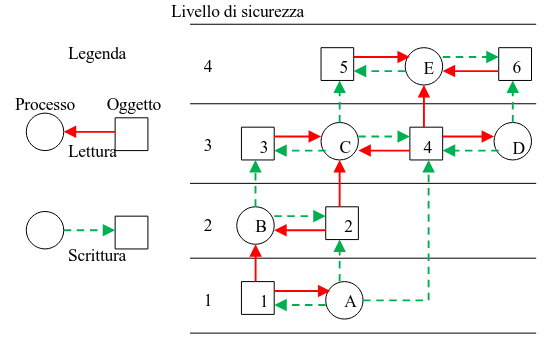
\includegraphics[width=0.8\textwidth]{/home/riccardoob/appunti/sistemi_operativi/images/14.png}
\end{figure}

Questo modello non è concepito per mantenere l'integrità dei dati ma per conservare segreti, è infatti ammesso sovrascrivere informazioni appartenenti a livelli superiori.

\subsubsection{Esempio - difesa cavalli di troia}

Si immagini un utente, Paolo, creatore del file \texttt{Fp} contenente una stringa riservata con permessi \texttt{r/w} solo per processi che appartengono a lui. Un utente ostile, Marco, ottenuto accesso al sistema, installa il file eseguibile \texttt{CT} e copia nel file system un file privato \texttt{Fm} che verrà utilizzato come "tasca posteriore".

Marco induce Paolo a eseguire il processo \texttt{CT}, che copia il contenuto di \texttt{Fp} in \texttt{Fm}, senza violare classiche regole di protezione (es. ACL).

Il modello, per prevenire attacchi di questo tipo, implementa 2 livelli di sicurezza, \textbf{privato} e \textbf{pubblico}:
\begin{itemize}
    \item ai processi e file di Paolo viene assegnato il livello \textit{riservato}
    \item ai processi e file di Marco viene assegnato il livello \textit{pubblico}
\end{itemize}

Quando il processo, avviato da Paolo con livello riservato, tenta di scrivere su \texttt{Fm} (pubblico) la proprietà \texttt{*} è violata e il tentativo è negato, nonostante ACL lo consenta.

La politica di sicurezza ha la precedenza sulle regole ACL.

\begin{figure}[H]
    \caption{Diagramma blocco cavallo di troia}
    \centering
    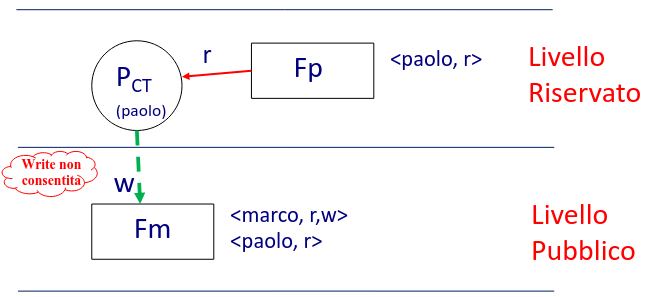
\includegraphics[width=0.8\textwidth]{/home/riccardoob/appunti/sistemi_operativi/images/15.png}
\end{figure}

\subsection{Modello Biba}

L'obiettivo di questo modello è l'integrità dei dati, diversamente dal Bell-La Padula.

\begin{itemize}
    \item \underline{proprietà di semplice sicurezza}: un processo in esecuzione al livello di sicurezza k può scrivere solo oggetti al suo livello o a livelli inferiori
    \item \underline{proprietà \texttt{*}} : un processo in esecuzione al livello di sicurezza k può leggere solamente oggetti al suol livello o a quelli superiori
\end{itemize}

Questo modello è il duale matematico del Bell-La Padula, quindi non sono utilizzabili contemporaneamente.

\subsection{Architettura dei sistemi ad elevata sicurezza}

\paragraph{Sistemi operativi sicuri o fidati} Sistemi per i quali è possibile definire formalmente dei requisiti di sicurezza.

\paragraph{Reference monitor} É un elemento di controllo realizzato a livello hardware che regola l'accesso dei soggetti agli oggetti sulla base di parametri di sicurezza.

\paragraph{Trusted computing base} Il RM ha accesso a una base di calcolo fidata (TCB) che contiene:
\begin{itemize}
    \item privilegi di sicurezza per ogni soggetto
    \item attributi (classificazione di sicurezza) di ciascun oggetto
\end{itemize}

\begin{figure}[H]
    \caption{Architettura sistemi ad elevata sicurezza}
    \centering
    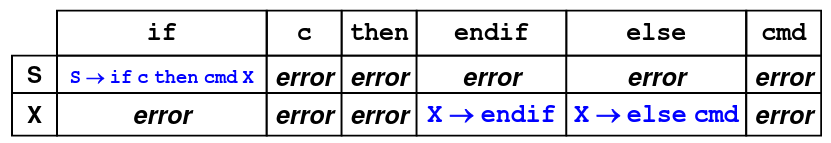
\includegraphics[width=0.8\textwidth]{/home/riccardoob/appunti/sistemi_operativi/images/16.png}
\end{figure}

\subsection{Sistemi fidati}

Il reference monitor impone le regole di sicurezza (Bell-La Padula) e ha le seguenti proprietà:

\paragraph{Mediazione completa} Le regole di sicurezza vengono applicate ad ogni accesso. Per motivi di efficienza, le soluzioni devono essere almeno parzialmente hardware.

\paragraph{Isolamento} il reference monitor e la base di dati sono protetti da modifiche non autorizzate.

\paragraph{Verificabilità} La correttezza del reference monitor deve essere provata, deve essere possibile dimostrare formalmente che il monitor impone le corrette regole di sicurezza e fornisce mediazione completa e isolamente.

Viene inoltre compilato un \textbf{audit file} dove vengono mantenuti gli eventi importanti per la sicurezza, come i tentativi di violazione alla sicurezza e le modifiche non autorizzate al nucleo di sicurezza.
















